\documentclass[fleqn,final]{beamer}
\mode<presentation>
{  \usetheme{I6dv} }
\usepackage{times}
\usepackage{etex}
\usepackage{amsmath,amssymb}
%\usepackage{sfmath} % for sans serif math fonts; wget http://dtrx.de/od/tex/sfmath.sty
\usepackage[english]{babel}
\usepackage[ansinew]{inputenc}
\usepackage[orientation=portrait,size=a0,scale=1,debug]{beamerposter}
\usepackage{booktabs,array}
\usepackage{listings}
%\usepackage{picins,graphicx}
\usepackage{xspace}
\usepackage{fp}
\usepackage{ifthen}
\usepackage[T1]{fontenc}
\usepackage{graphicx}
\usepackage{tikz,colortbl,pgf,pgfarrows,pgfnodes,pgfautomata,pgfheaps,pgfshade,eurosym, dsfont}
\usepackage{tcolorbox}
\listfiles
\newcommand*{\signstream}{SignStream\texttrademark\xspace}
\newcommand{\WichtigFarbe}{\color{red}}%
\newcommand{\TextFarbe}{\color{black}}%
\newcommand{\Pheight}{\rule[-5mm]{0cm}{1cm}}

\definecolor{darkblue}{rgb}{0.28,0,0.60}
\definecolor{hblue}{rgb}{0.70,0.7,1}
\definecolor{NR0}{rgb}{1,1,1}
\definecolor{NR1}{rgb}{1,1,0.8}
\definecolor{NR2}{rgb}{1,1,0.5}
\definecolor{NR3}{rgb}{1,1,0.25}
\definecolor{NR4}{rgb}{1,1,0.0}
\definecolor{NR5}{rgb}{1,0.75,0.0}
\definecolor{NR6}{rgb}{1,0.5,0.0}
\definecolor{NR7}{rgb}{1,0.25,0.0}
\definecolor{NR8}{rgb}{1,0,0.0}

\setbeamertemplate{navigation symbols}{}
\setbeamerfont{title}{series=\bfseries}
%\setbeamercolor{frametitle}{fg=UTblue}
\setbeamerfont{frametitle}{series=\bfseries}
\setbeamertemplate{frametitle}
{
\begin{centering}
\insertframetitle\vspace*{-4mm}\par
\end{centering}
}

\newcommand{\convD}{\stackrel{\text{d}}{\longrightarrow}}
\newcommand{\E}{\text{E}\,}
\newcommand{\var}{\text{V}\,}

\title{\huge Performance of Empirical Best Predictor in Informative Samples - A Monte Carlo Simulation}
\author{\large Felix Skarke, Enno Tammena, Christian Koopmann}
\institute{Freie Universit{\"a}t Berlin, Humboldt Universit{\"a}t zu Berlin}

\date{today}
\begin{document}

\begin{frame}

%
%------------------------------------------------------ ------------------------------------------------------
%
\small
\begin{columns}[t] % Wechsel in die Spaltenumgebung

\begin{column}{.3\linewidth} 
\begin{block}{Motivation  \Pheight}
\begin{itemize}
\item Use of direct estimators in domains of interest with insufficient sample size can lead to unreliable results  \\
$\Rightarrow$ Using small area methods like EBP (Empirical Best Predictor) approach can be preferable \\
\vskip .5cm
\item  In model-based inference normally the sampling design is assumed to be uninformative (e.g. simple random sampling):\\ $P(s|y)=P(s),\;\; \forall y\in \mathbb{R}^N,\; \forall s$
\vskip .5cm
\item When complex designs are used for sampling (practical reasons, special interest in small subpopulation), ignoring weights can lead to biased estimators \\
$\Rightarrow$ Use of direct estimators like weighted Gini\\

\vskip .5cm
\item Problem: sampling weights cannot be used directly in the EBP approach because of non-linearity of indicator
\vskip .5cm
\item The aim of this study is to evaluate the performance of EBP relative to direct estimation under a complex sampling design
\end{itemize}

\end{block}
\end{column}

%
%------------------------------------------------------ ------------------------------------------------------
%

\begin{column}{.3\linewidth}
\begin{block}{The Gini: a measure for inequality\Pheight}
\begin{minipage}{0.5\textwidth}
\begin{figure}[ht]
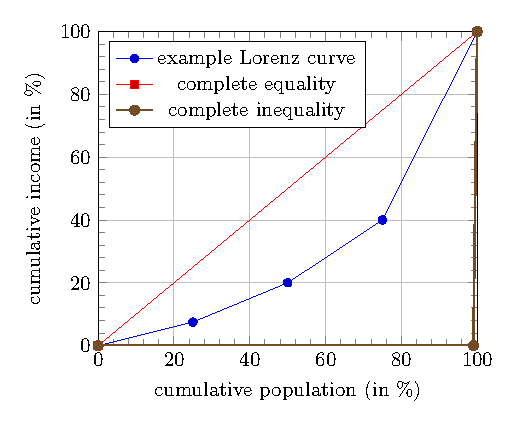
\includegraphics[scale=1.5]{Lorenz.pdf}
\end{figure}
\end{minipage}%
\begin{minipage}{.5\textwidth}
\begin{itemize}
\item The Gini coefficient is used to measure inequality of distribution (e.g. income, wealth) in a society
\item It is defined as the area between the Lorenz curve and the $45^{\circ}$ line (=A) in relation to the area beneath the $45^{\circ}$  line (=A+B), where B is the area under the Lorenz curve  
\end{itemize}
\end{minipage}%
\end{block}
\vskip .5cm
\centering
\begin{tcolorbox}
Therefore it can be expressed as:
\begin{equation*}
G=A/(A+B)=2A=1-2B
\end{equation*}
\end{tcolorbox}
\end{column}

%
%------------------------------------------------------ ------------------------------------------------------
%

\begin{column}{.3\linewidth}
 \begin{block}{The Gini: unweighted and weighted \Pheight}
The Gini coefficient can be expressed without a direct reference to the Lorenz curve:\\
\vskip 0.5cm
\textbf{unweighted version}
\begin{tcolorbox}
\begin{equation*}
\hat{G}={\frac {2\sum_{j=1}^{n}\;jy_{j}}{n\sum _{j=1}^{n}y_{j}}}-{\frac {n+1}{n}}
\end{equation*}
\end{tcolorbox}
\vskip 0.5cm
\textbf{weighted version}
\begin{tcolorbox}
\begin{equation*}
\hat{G}=100\Bigg[{\frac {2\sum_{j=1}^{n}\;(w_{j}y_{j}\sum_{l=1}^{j}\;w_{l})-\sum_{j=1}^{n}\;w_{j}^{2}y_{j}}{(\sum_{j=1}^{n}\;w_{j})\sum_{j=1}^{n}\;(w_{j}y_{j})}-1}\Bigg]
\end{equation*}
\end{tcolorbox}
\vskip 0.5cm
{\fontencoding{U}\fontfamily{futs}\selectfont\char 66\relax} Using weights in direct estimators can be important, if a complex sampling design is used. 
\end{block}
\end{column}

%
%------------------------------------------------------ ------------------------------------------------------
%

\end{columns}


\begin{columns}[t]


%
%------------------------------------------------------ ------------------------------------------------------
%


  
\begin{column}{.3\linewidth}
\begin{block}{Empirical Best Predictor \Pheight}
\underline{Random Effects model}:\\
\vskip 1.5cm
\scalebox{1.2}{$y_{ij}=x_{ij}\prime\beta+u_{i}+e_{ij},\;\;\;j=1,\dots,n_{i},\;\;i=1,\dots,D$} \\
\vskip 1.0cm
,where $u_{i}\sim iid\mathcal{N}(0,\sigma_{u}^2)$ and $e_{ij}\sim iid\mathcal{N}(0,\sigma_{e}^2)$ \\
\vskip 2cm
\textbf{Estimation of model}:
\vskip .5cm
\begin{enumerate}
\item estimate $\hat{\beta},\hat{\sigma}_{u}^2,\hat{\sigma}_{e}^2,\hat{u}_{i},\hat{\gamma}_{i}=\frac{\hat{\sigma}_{u}^2}{\hat{\sigma}_{u}^2+\frac{\hat{\sigma}_{e}^2}{n_{i}}}$ from sample
\item generate $e_{ij}^*\sim\mathcal{N}(0,\hat{\sigma}_{e}^2)$ and $u_{i}^*\sim\mathcal{N}(0,\hat{\sigma}_{u}^2(1-\hat{\gamma}_{i}))$ for L pseudo-populations: \[y_{ij}^{*(l)}=x_{ij}\prime\hat{\beta}+\hat{u}_{i}+u_{i}^*+e_{ij}^*\]\\
$\Rightarrow$ obtain an indicator of interest in each domain for every pseudo-population
\item calculate $\hat{\theta}_{i}^{EBP}=\frac{1}{L}\sum_{l=1}^{L}\hat{\theta}_{i}^{(l)}$ for each domain
\end{enumerate}

\end{block}
\end{column}
%
%------------------------------------------------------ ------------------------------------------------------
% Folie 5
   
\begin{column}{.3\linewidth}

\begin{block}{MSE estimation \Pheight}
Since analytical approximations of the MSE are difficult or even impossible to derive in the case of nonlinear indicators like the Gini. The MSE is approximated using a bootstrap procedure:
\begin{enumerate}
\item Fit the model to the sample data and therefore obtain estimates for $\beta, \sigma_{u}^2 and \sigma_{e}^2$
\item Generate $u_{i}^*\sim iid \mathcal{N}(0,\hat{\sigma}_{u}^2)$ and  $e_{ij}^*\sim iid \mathcal{N}(0,\hat{\sigma}_{e}^2)$ independently for every domain and every person in the population
\item Construct a superpopulation using the generated error terms and the population covariates
\[y_{ij}^*=x_{ij}\prime\hat{\beta}+u_{i}^*+e_{ij}^*\]
\item Draw B bootstrap populations from the superpopulation and calculate $\theta_{i}^{*b}$ in every domain for each of the populations
\item Draw a bootstrap sample from every population, implement the EBP and estimate $\hat{\theta}_{i}^{*b}$
\item Finally estimate the MSE per domain by: 
\[\hat{MSE}(\hat{\theta}_{i})=\frac{1}{B}\sum_{b=1}^B (\hat{\theta}_{i}^{*b}-\theta_{i}^{*b})^2\]
\end{enumerate}
\end{block}
\end{column}    



%
%------------------------------------------------------ ------------------------------------------------------
% Folie 6 

  % 


\begin{column}{.3\linewidth}

 \begin{block}{Data and Sampling \Pheight}

Assume the following scenario: 
\begin{enumerate}
\item Stratified sample ($i$ income groups nested in SMAs) with data on y and X
\begin{itemize}
\item In each SMA, an equal number of observations per income group is sampled such that:
\begin{itemize}
\item Sample size $n_{SMA}$ per SMA is proportional to  $N_{SMA}$ 
\item Smaller income groups are oversampled
\end{itemize}
\item Weights differ between income groups and SMAs
$\rightarrow frequency weights_{SMA, income group} = {\frac {N_{SMA,income group}} {n_{SMA}/i}} $
\end{itemize}
\item Population data on X on SMA level is available


\begin{itemize}
\item approach is generalizable to other forms of sampling, where certain groups are over- or undersampled in a stratified setting
\end{itemize} 

 \item Dataset: EUSILC Data as provided by the emdi package
\begin{itemize}

\item to achieve a sufficient population size $N$, randomly duplicate observations between 1 and 8 times
\item add $\varepsilon$ to the dependent variable of duplicated observations, where  $\varepsilon \sim N(0,5000)$
\end{itemize} 
\end{enumerate}

\end{block}
\end{column} 



%
%------------------------------------------------------ ------------------------------------------------------
%
  
\end{columns}  



\begin{columns}[t]

%
%------------------------------------------------------ ------------------------------------------------------
% Folie 6 

  % 


\begin{column}{.3\linewidth}


\begin{block}{Implementation \Pheight}
\begin{itemize}

\item take an initial random sample of size $n$ with same number ($g$) of observations from each income group 
\item calculate $n_{SMA}$
\item calculate $frequency weights$
 
\item for 1:s \{
\begin{enumerate}  % F�r Aufz�hlungen
\item split population by SMA, take a sample of $n_{SMA} / 5$ from each income group
\item estimate $\widehat{Gini}_{direct\_unweighted}, \widehat{Gini}_{direct\_weighted}$ per SMA
\item estimate $\widehat{Gini}_{EBP\_unweighted}$  based on $l$ pseudo-populations per SMA
\item estimate $\widehat{MSE}_{Gini_{unweighted\_EBP}}$ based on $b$ bootstraps per SMA
\item expand the sample by frequency weights
\item estimate $\widehat{Gini}_{EBP\_weighted}$  based on $l$ pseudo-populations per SMA
\item save the results per SMA
\end{enumerate}
\}
calculate $Gini_{SMA}$ based on population
 
\item calculate quality measures per SMA
	\begin{itemize}
		\item $MSE_{SMA} = \sum_{i = 1}^{s} (\widehat{Gini}_{SMA} - Gini_{SMA})^2$
		\item $RelBias_{SMA} = \sum_{i = 1}^{s} (\widehat{Gini}_{SMA} - Gini_{SMA})/Gini_{SMA}$
	\end{itemize}
\item Parameters: $N=112644, s=250, g=2000, n=10000, l=50, b=10, SMA=district, i=5$
\end{itemize}
\end{block}



 
\end{column}

%
%------------------------------------------------------ ------------------------------------------------------
% 10 


\begin{column}{.3\linewidth}

\begin{block}{RMSE of weighted and unweighted EBP\Pheight}
\begin{center}
	\begin{figure}
		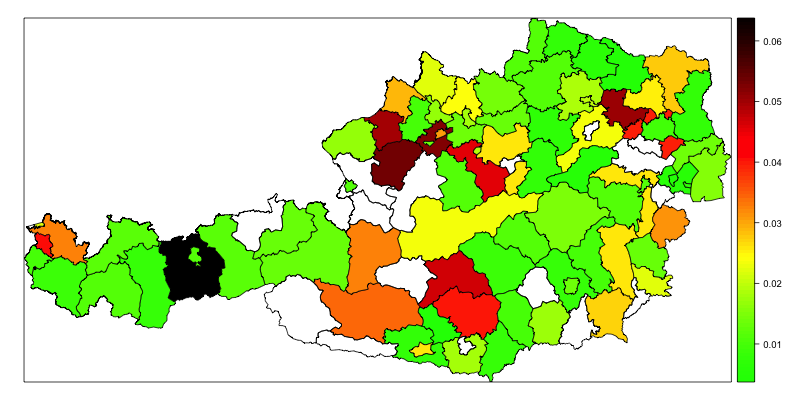
\includegraphics[width=0.9\textwidth]{EBPWeightedRMSE}
		\caption{RMSE of Weighted EBP per Domain}
	\end{figure}
		\begin{figure}
		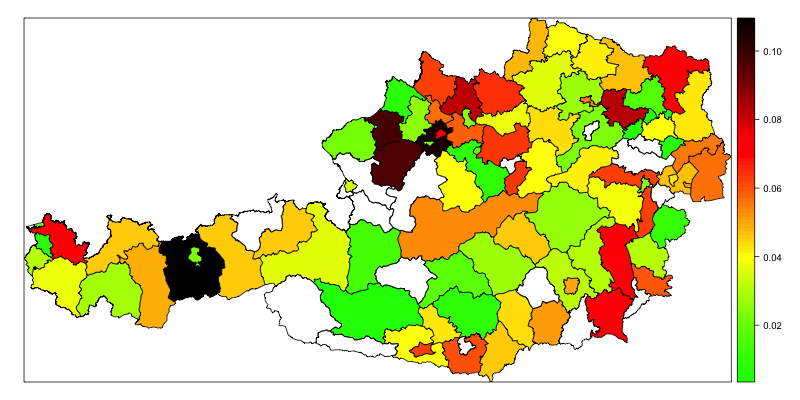
\includegraphics[width=0.9\textwidth]{EBPUnweightedRMSE}
		\caption{RMSE of Unweighted EBP per Domain}
	\end{figure}
\end{center}

\end{block}

\end{column}

%
%------------------------------------------------------ ------------------------------------------------------
% 11

\begin{column}{.3\linewidth}

\begin{block}{Domain Level MRE and RMSE of Estimators \Pheight}
\begin{center}
	\begin{figure}
		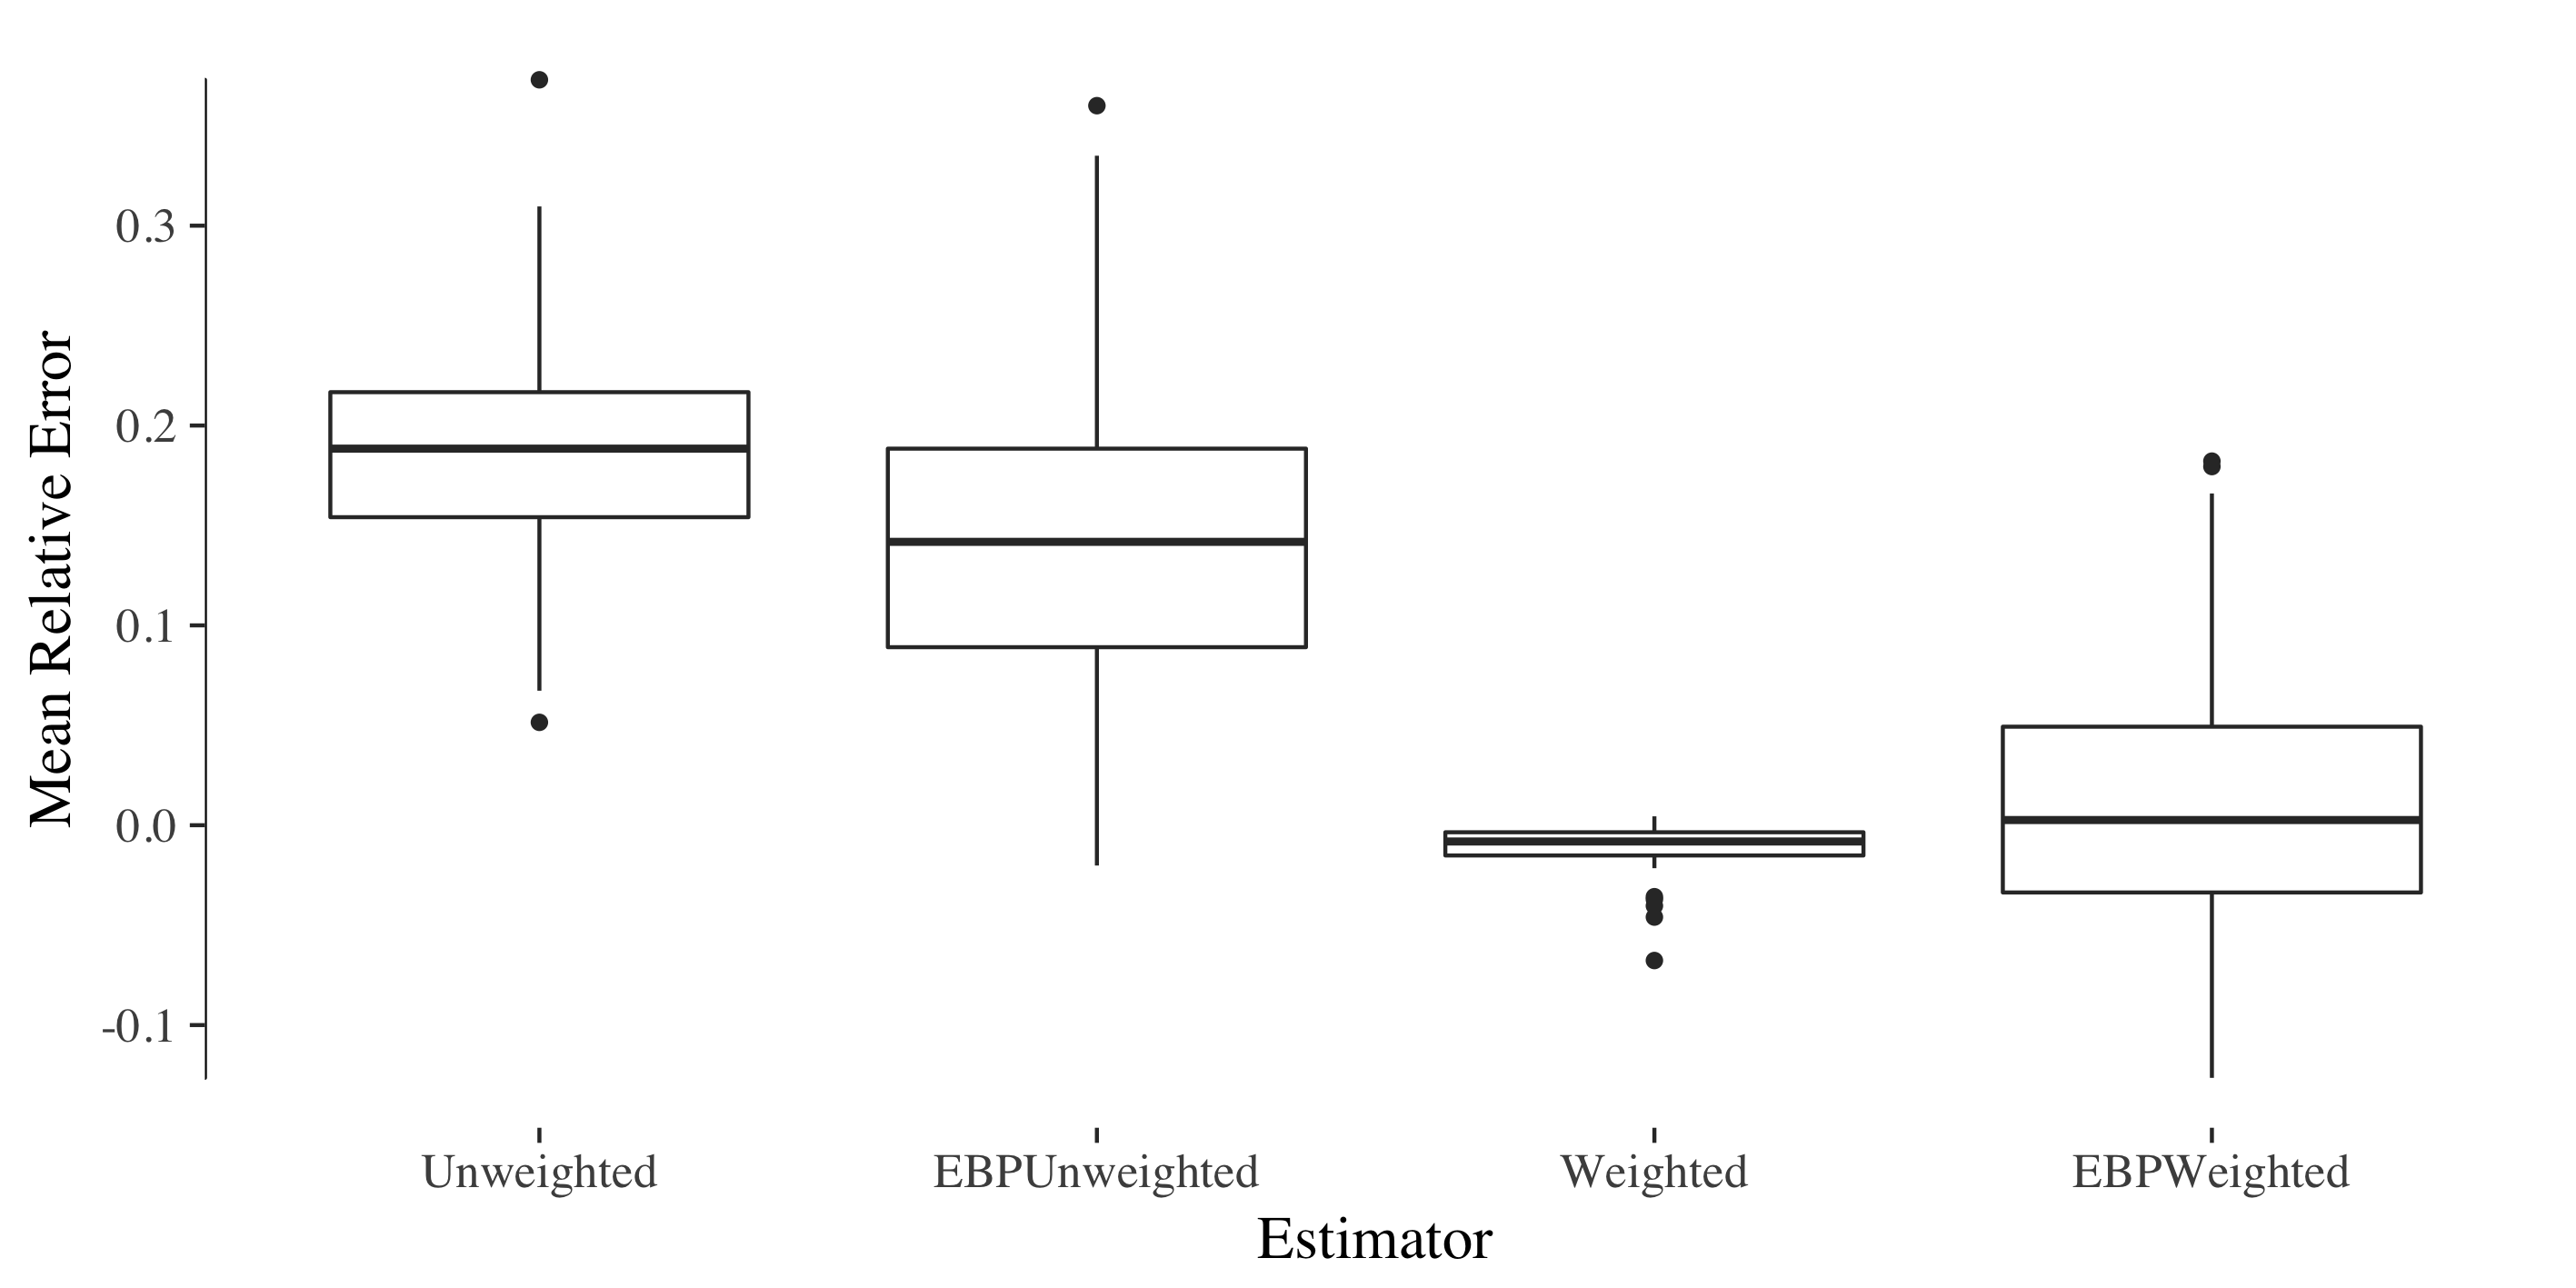
\includegraphics[width=0.9\textwidth]{BoxPlotMREByDomain}
		\caption{Boxplot of Relative Bias on Domain Level}
	\end{figure}
		\begin{figure}
		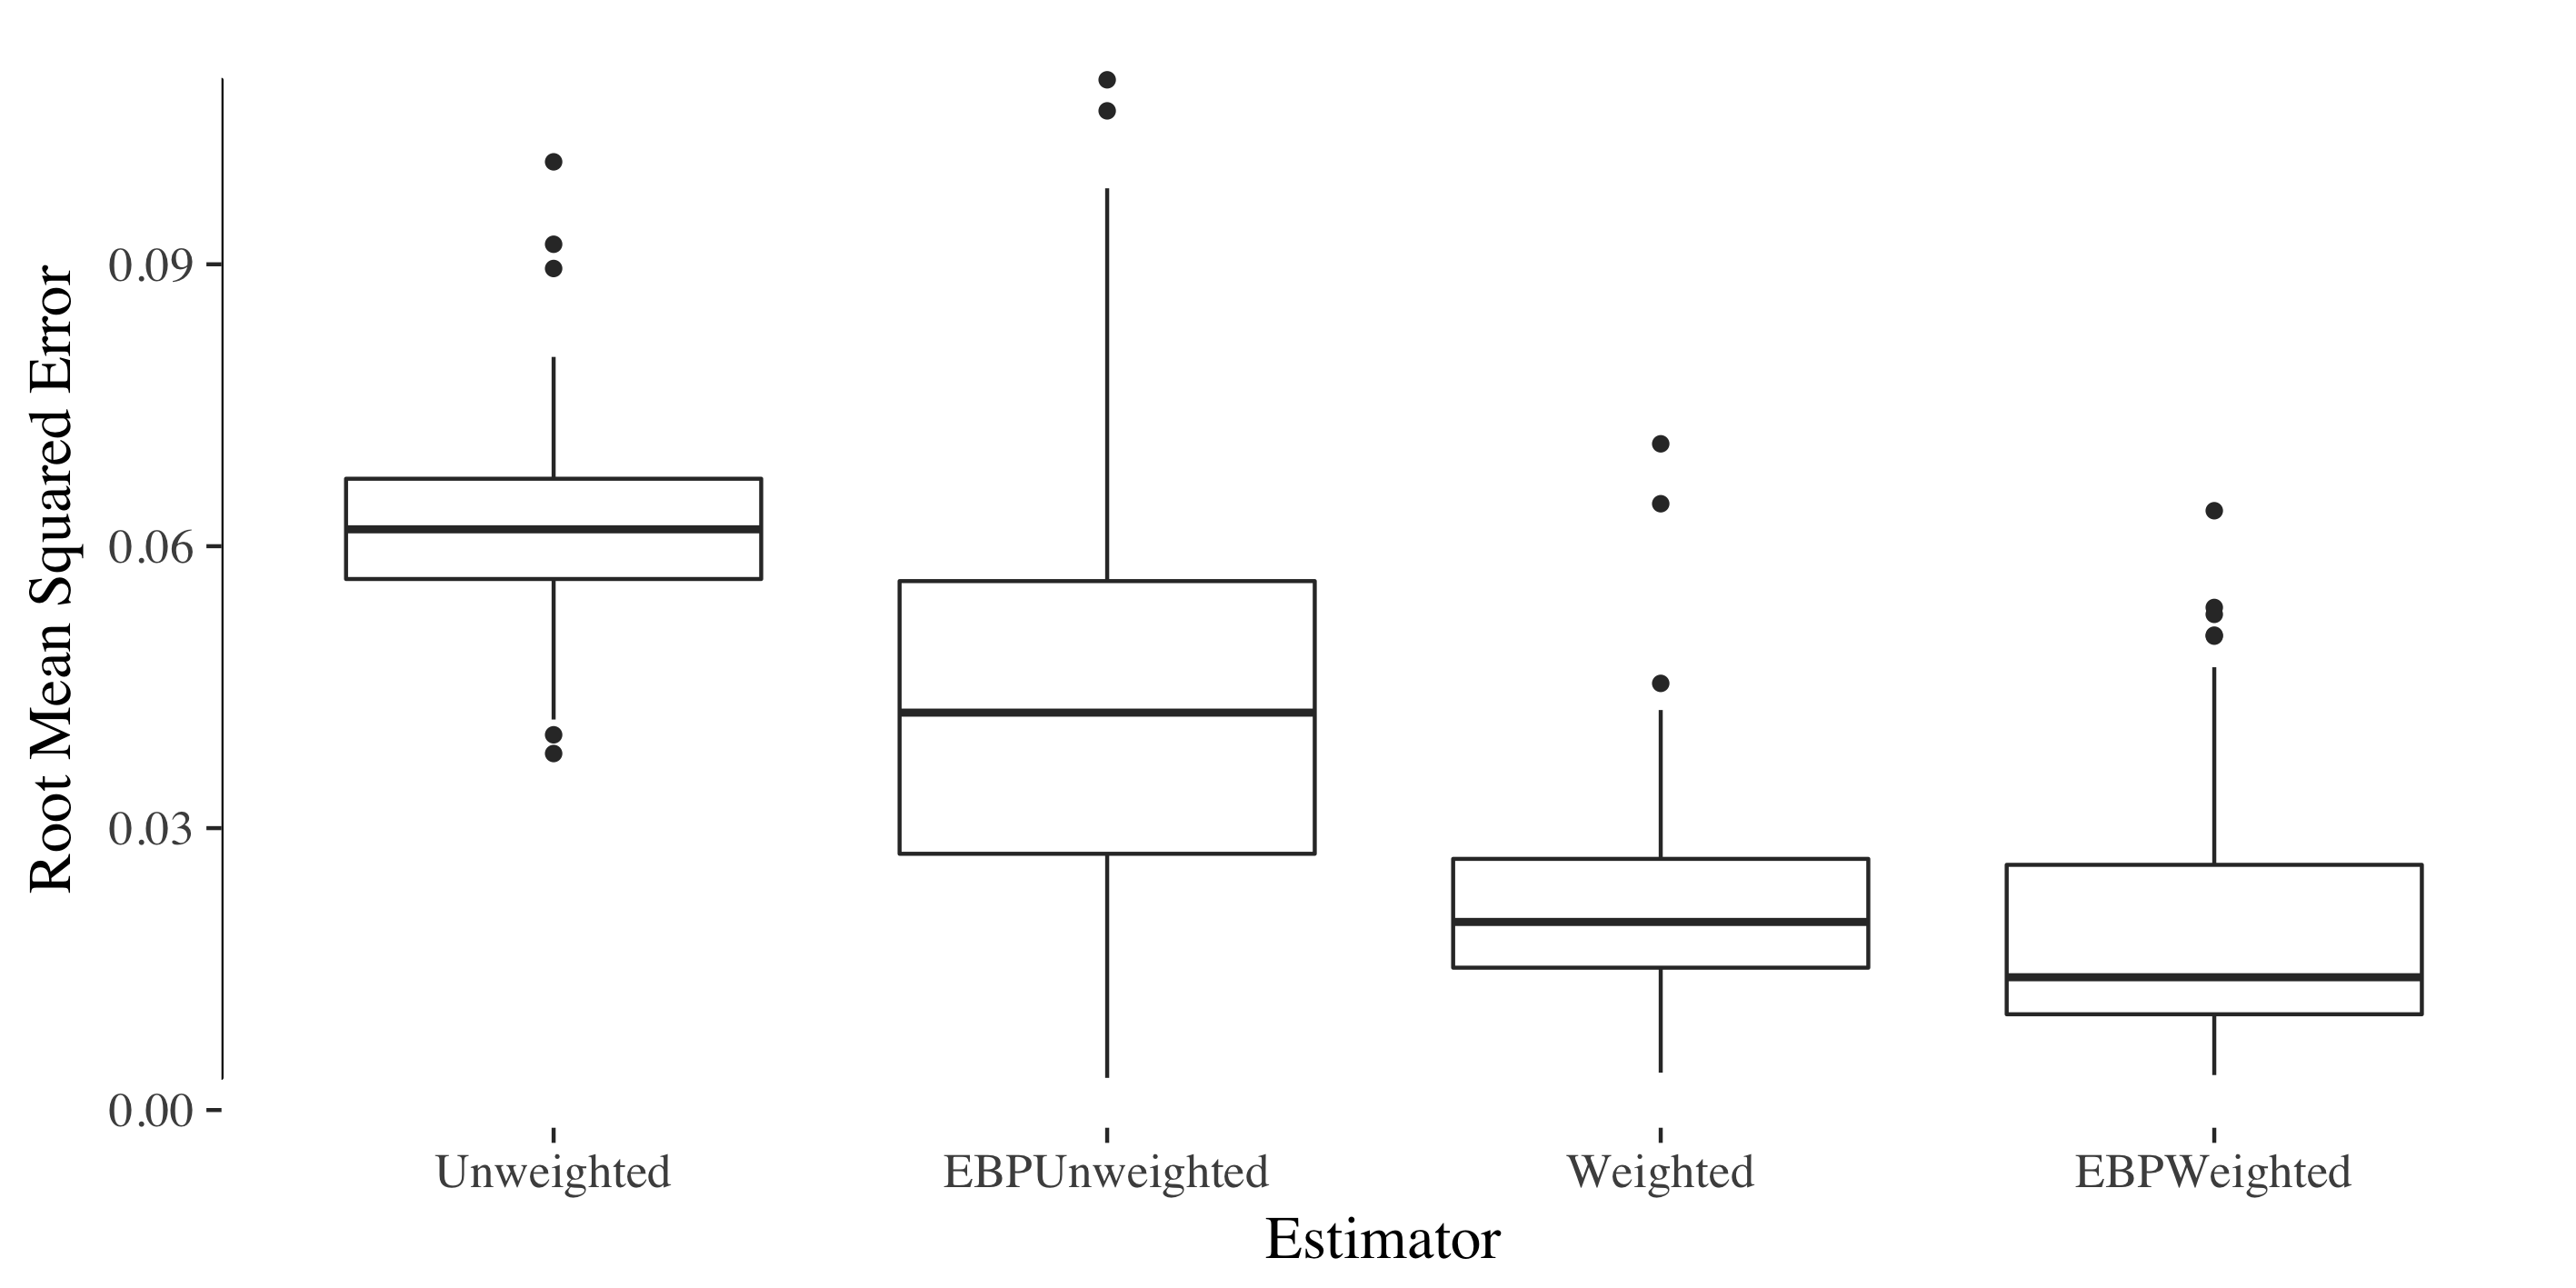
\includegraphics[width=0.9\textwidth]{BoxPlotRMSEByDomain}
		\caption{Boxplot of RMSE on Domain Level}
	\end{figure}
\end{center}
\end{block}

\end{column}
\end{columns}

\begin{columns}[t]
%
%-------------------------------------------------------------------------------------------------------------
% 12

\begin{column}{.3\linewidth}


  \begin{block}{ Accuracy of inbuilt MSE estimator \Pheight}
	\begin{center}
	\begin{figure}
		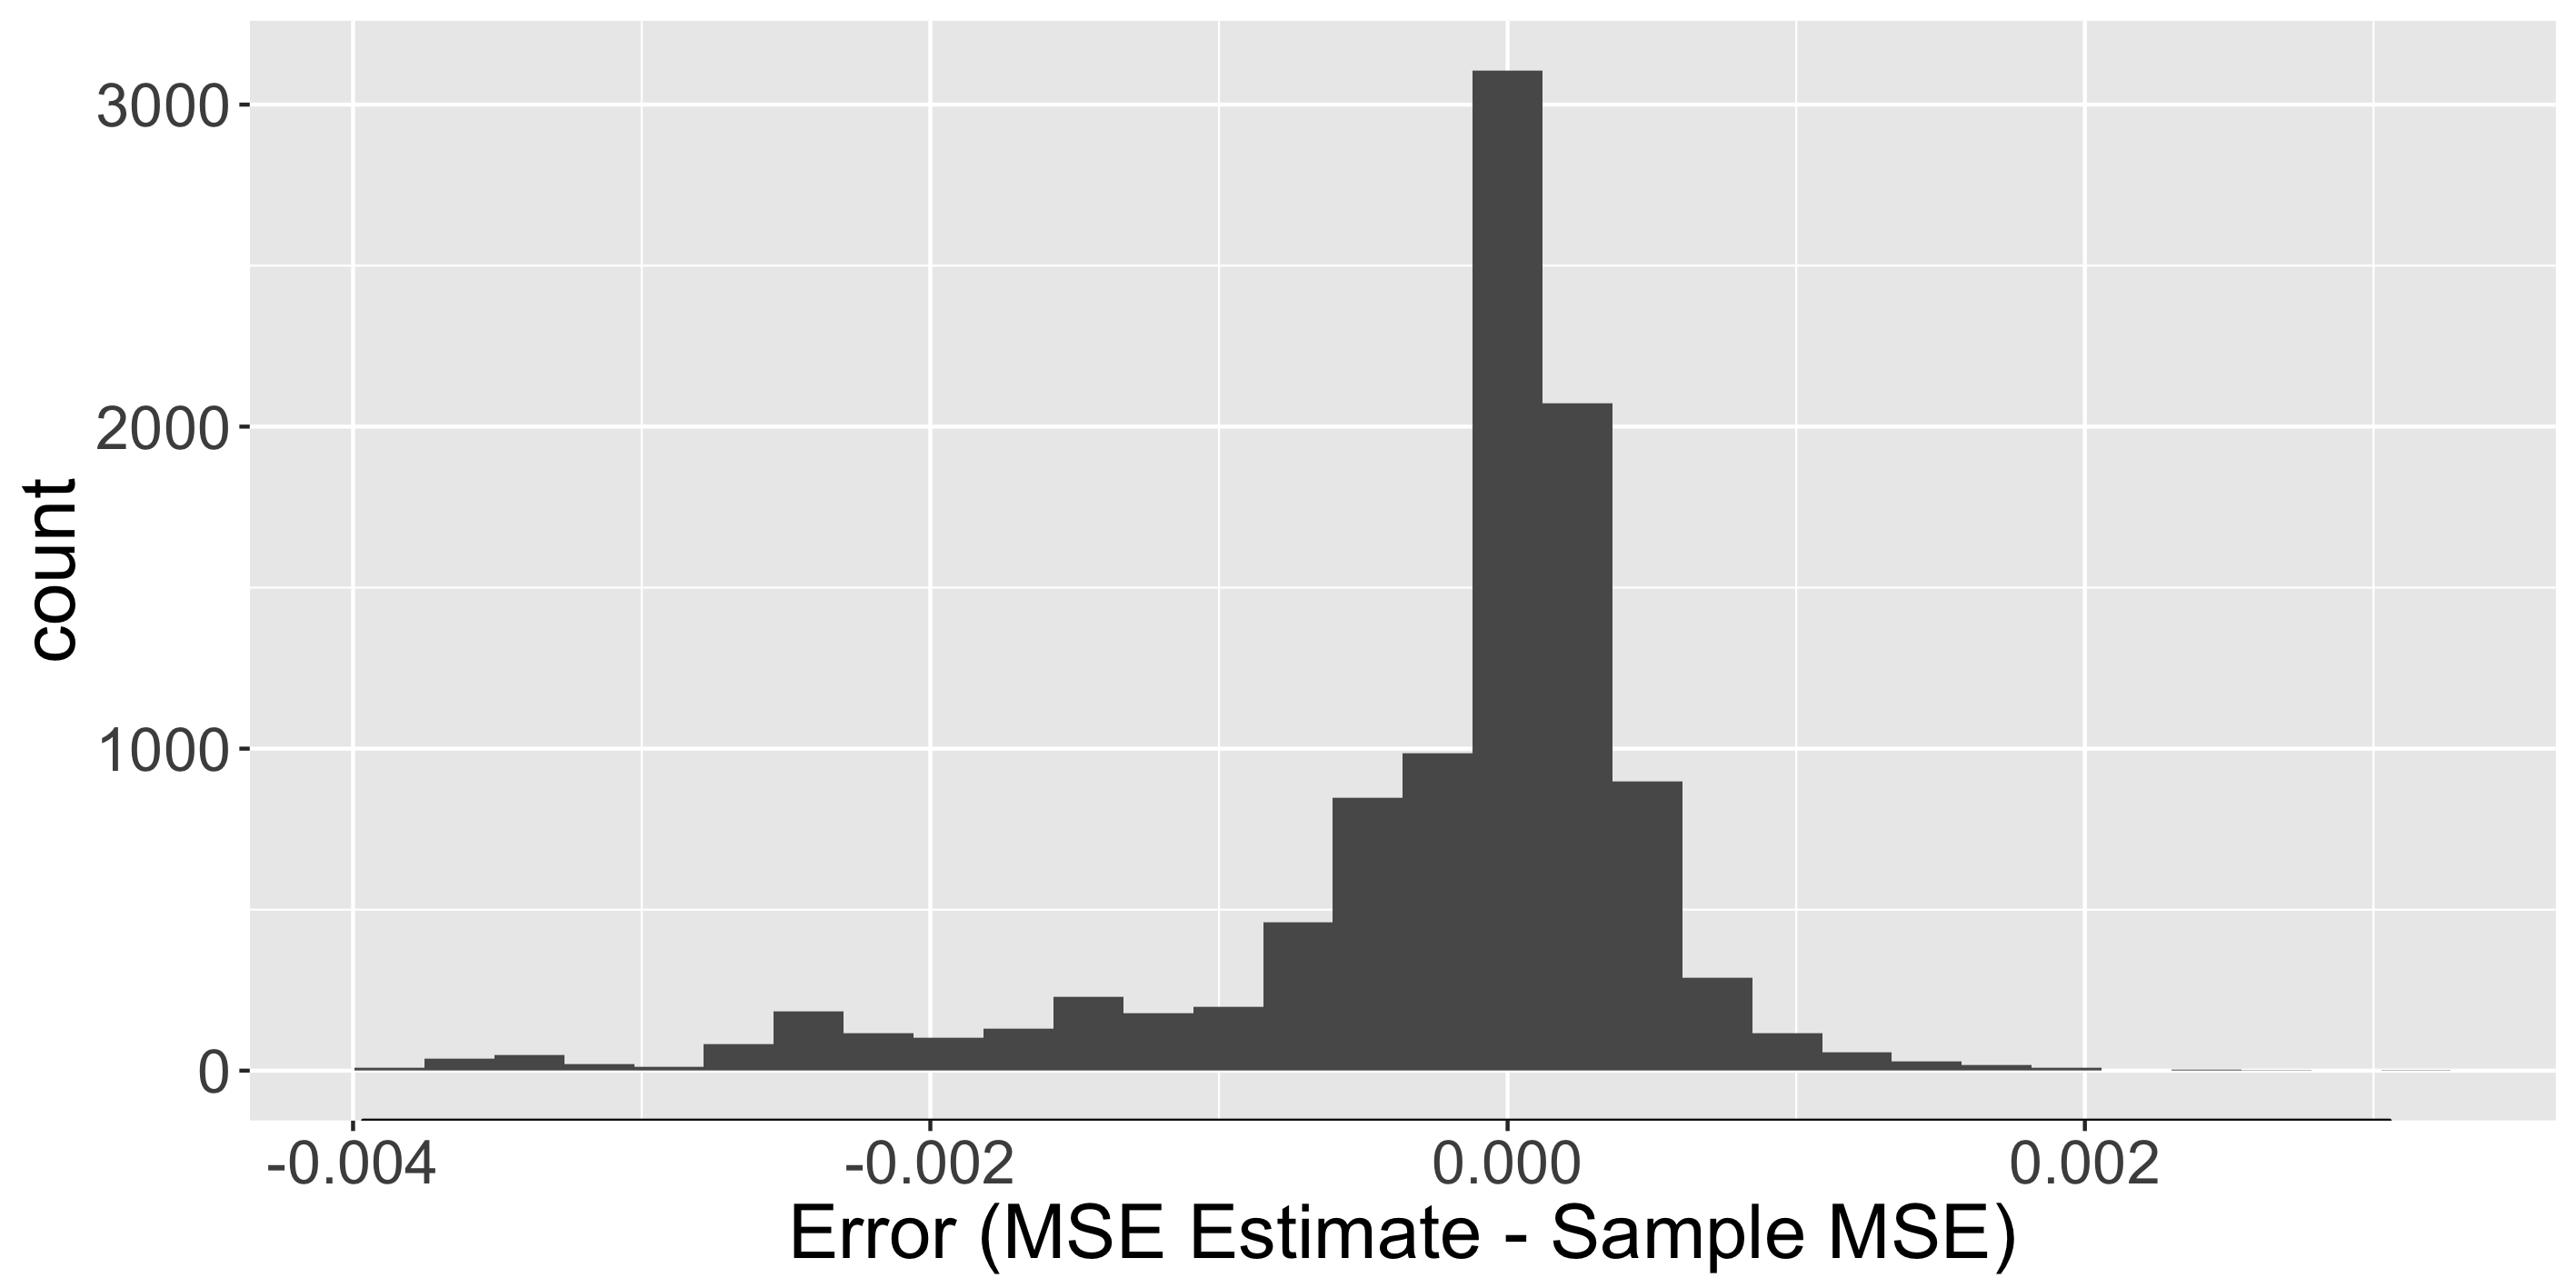
\includegraphics[width=0.9\textwidth]{HistogramMSEEstimate}
		\caption{Histogram of Difference between EBP MSE estimator and the sample MSE across iterations}
	\end{figure}
	\end{center}
	\textbf{Observations:}
	\begin{itemize}
	\item Bootstrap estimator agrees quite well with sample MSE
	\item Slightly more likely to underestimate sample MSE
	\end{itemize}
   \end{block}
\end{column}

%
%------------------------------------------------------ ------------------------------------------------------
%

\begin{column}{.3\linewidth}
\begin{block}{Conclusions \Pheight}
\textbf{Conclusions:}
\begin{itemize}
	\item Unweighted direct estimator and EBP are both biased unlike their weighted versions.
	\item Weighting substantially increase accuracy for both estimators.
	\item Relative accuracy advantage of EBP over direct estimation is much larger in the unweighted case.
	\item Weights  can be included in EBP estimation  by expanding the sample using frequency weights.
\end{itemize}
\textbf{Future Research:}
\begin{itemize}
	\item Explore alternative ways of including weights into EBP estimation.
	\item Analyse alternative sampling designs.
\end{itemize}
\end{block}
\end{column}
%
%----------------------------------------------------------
%
\begin{column}{.3\linewidth}
\begin{block}{Bibliography \Pheight}
\begin{thebibliography}{9}
\bibitem {A} Alfons, A., and Templ, M. (2013) Estimation of Social Exclusion Indicators from Complex Surveys: The R Package laeken. Journal of Statistical Software, 54, 1-25. 
\bibitem {G} Guadarrama, M., Molina, I., and Rao, J.N.K. (2016) Small area estimation of general parameters under complex sampling designs. UC3M Working Papers, Statistics and Econometrics, 16-05.
\bibitem {M} Molina, I., and Rao, J.N.K. (2010) Small area estimation of poverty indicators. Canandian Journal of Statistic, 38, 369-385.
\bibitem {V} Verret, F., Rao, J.N.K, and Hidiroglou, M.A. (2015) Model-based small area estimation under informative sampling. Survey Methodology, 41.2, 333-347.
\end{thebibliography}


\end{block}
\end{column}

\end{columns}


\end{frame}


\end{document}

